\subsection{Sprint 2: da 2024-04-22 a 2024-05-06}
\par A causa delle difficoltà riscontrate nel primo \glossario{sprint}, il team ha convenuto di valutare strumenti alternativi a \glossario{GitHub}, con l'obiettivo di migliorare l'organizzazione delle attività e la gestione di progetto. Inoltre, il gruppo ha pianificato lo studio delle tecnologie proposte dalla \glossario{Proponente} e l'aggiornamento della documentazione.

\subsubsection{Obiettivi}
\begin{itemize}
  \item Valutazione del passaggio a un \glossario{Issue Tracking System} che offra funzionalità più orientate alla gestione dei compiti rispetto a \glossario{GitHub};
  \item Progettazione dettagliata del \glossario{dizionario dati};
  \item Studio delle tecnologie per l'interazione tra il \glossario{dizionario dati} e la richiesta dell'utente in linguaggio naturale;
  \item Conversione in \glossario{LaTeX} del documento di \AdR;
  \item Studio della composizione del \glossario{prompt} da fornire in output all'utente;
  \item Stesura iniziale del \PdQ;
  \item Aggiornamento dei documenti \PdP, \NdP, \Gls\ e \AdR;
  \item Stesura verbali interni ed esterni.
\end{itemize}

\begin{figure}[H]
  \centering
  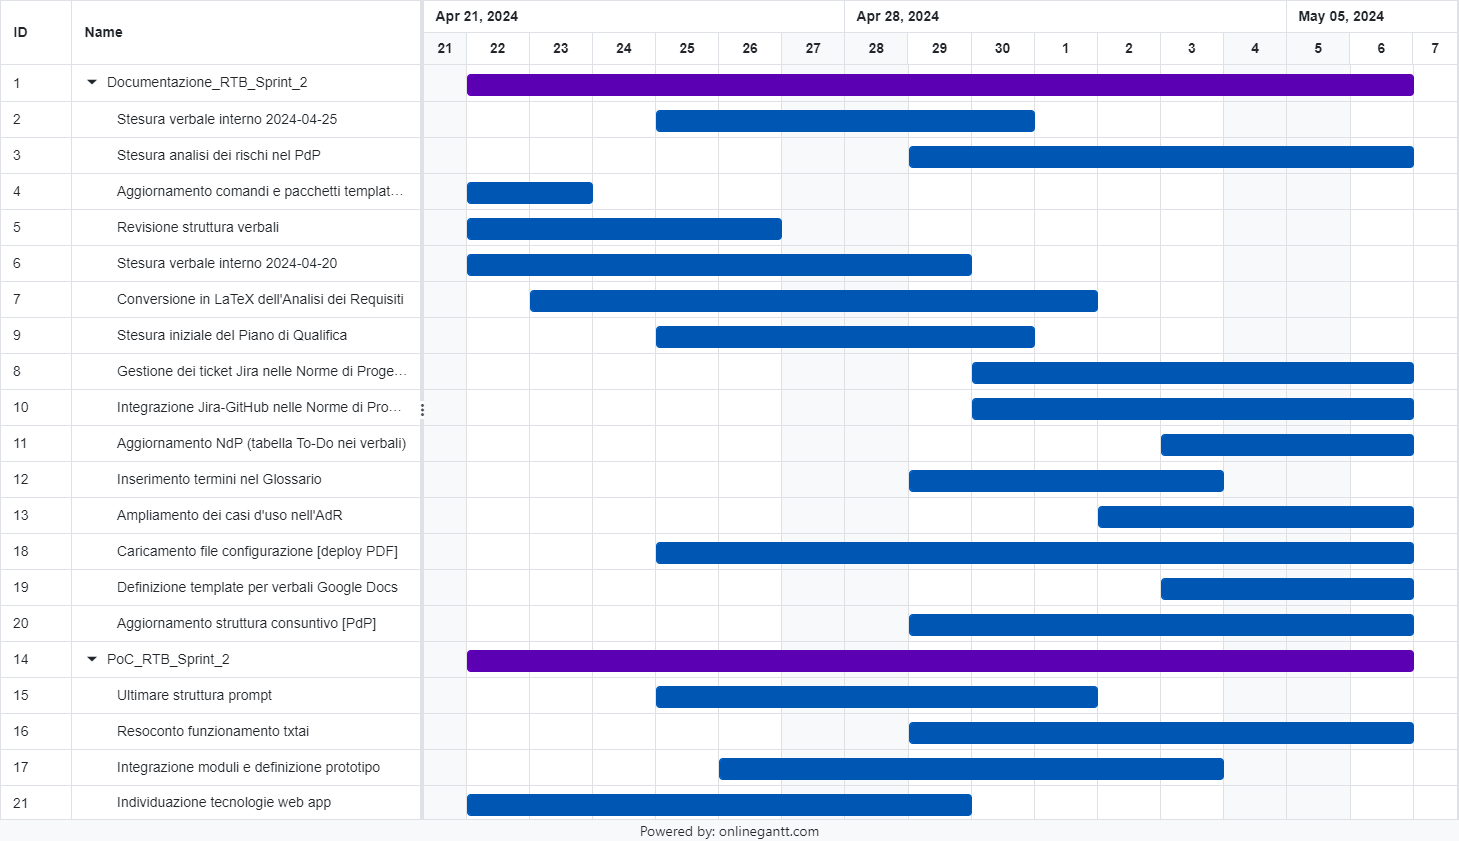
\includegraphics[width=0.90\textwidth]{assets/Pianificazione/Sprint-2/gantt.png}
  \caption{Sprint 2 - Diagramma di Gantt}\label{fig:sprint-2-gantt}
\end{figure}